\chapter{Topic Modeling}
\label{Chapter3}
\section{Topic Modeling là gì ?}
\begin{figure}[h!]
	\centering
	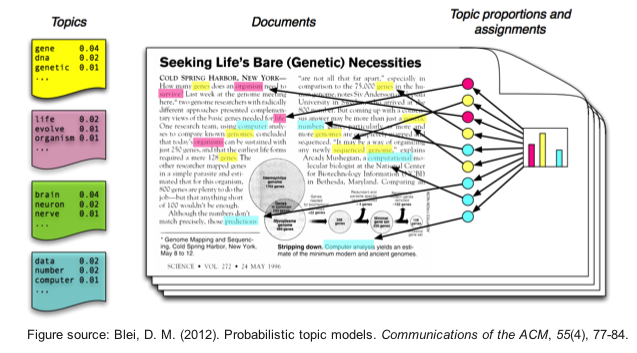
\includegraphics[width=1\textwidth]{
		topicModeling.png
	}
	\caption[Topic Modeling]{
		Topic Modeling   \cite{WEBSITE:11}
	}
\end{figure}
Topic modeling hay Mô hình hóa chủ đề là một kĩ thuật học máy tự động phân tích dữ liệu văn bản để xác định các từ cụm cho một tập hợp các tài liệu. Điều này được gọi là học máy 'không giám sát' vì nó không yêu cầu dữ liệu  được con người phân loại trước đây.

Ý tưởng về các topic models xoay quanh quá trình sắp xếp các văn bản vào những dạng chủ đề, khái niệm. 

Mỗi chủ để được biểu diễn dưới dạng là tập hợp của các từ/thuật ngữ có trong kho văn bản.

Nếu chúng xuất hiện cùng với nhau các từ/thuật ngữ này sẽ biểu thị, tượng trưng cho một chủ đề hoặc khái niệm cụ thể. Chúng ta có thể dễ dạng phân biệt các chủ đề với nhau nhờ ngữ nghĩa của các thuật ngữ đó

Tuy nhiên, các chủ đề thường có sự chồng chéo nhất định trên dữ liệu. Các topic models sẽ cực kỳ hữu ích trong việc tóm tắt, rút gọn khối lượng lớn tài liệu, văn bản để trích xuất, mô tả các khái niệm chính nhất. Chúng cũng hữu ích trong việc trích xuất các đặc trưng từ dữ liệu văn bản để nắm bắt các pattern tiềm ẩn trong dữ liệu đó. \cite{WEBSITE:12}



\section{Các kỹ thuật sửu dụng trong Topic Modeling}

Có nhiều kỹ thuật khác nhau để mô hình hóa chủ đề văn bản và hầu hết chúng liên quan đến một số dạng phân tách ma trận

Một số kỹ thuật như \cite{WEBSITE:11}:

\begin{enumerate}
	\item \textbf{Latent Semantic Analysis  (LSA) - Phân tích ngữ nghĩa tiềm ẩn} :sử dụng các phương pháp phân tách ma trận, cụ thể hơn là phân tách các giá trị đơn lẻ.
	\item \textbf{Latent Dirichlet Allocation (LDA) - Phân bố Dirichlet tiền ẩn}: một kỹ thuật sử dụng mô hình xác suất tổng quát trong đó mỗi mẫu tài liệu bao gồm một sự kết hợp của một số chủ đề và mỗi thuật ngữ hoặc từ có thể được gán cho một chủ đề cụ thể.
\end{enumerate}

\subsection{Latent Semantic Analysis (LSA)}

LSA (Phân tích ngữ nghĩa tiềm ẩn) còn được gọi là LSI (Chỉ số ngữ nghĩa tiềm ẩn) LSA sử dụng mô hình túi từ (BoW). 
Hàng và cột đại diện cho tài liệu. \\
LSA học các chủ đề tiềm ẩn bằng cáchsử dụng các phương pháp phân tách ma trận, cụ thể hơn là phân tách các giá trị đơn lẻ.

\textbf{Singular Value Decomposition(SVD)}
SVD là một phương pháp phân tích ma trận thành nhân tử đại diện cho một ma trận trong tích của hai ma trận \ref{equa1} \cite{WEBSITE:13}

\begin{equation}
	M=U \sum V^* \label{equa1}
\end{equation}
Trong đó:
\begin{itemize}
	\item M: là ma trận cỡ mxm\\
	\item U: là ma trận cỡ mxn phía bên trái\\
	\item V: là ma trận cỡ mxn phía bên phải\\
	\item V*: là ma trận chuyển vị của ma trận V\\
\end{itemize}

\textbf{Thực nghiệm thuật LSA sử dụng Gensim} \cite{WEBSITE:13}
\begin{enumerate}
	\item \textbf{Import các thư viện cần thiết}
		\lstinputlisting[style=codePython]{"Code/dependencies1.py"}
	\item \textbf{Load dữ liệu mẫu}:
		\lstinputlisting[style=codePython]{"Code/loadData.py"}
	
	\item \textbf{Tiền xử lý dữ liệu}:
		\lstinputlisting[style=codePython]{"Code/preprocessing.py"}
		
	\item \textbf{Chuẩn bị các dữ liệu dạng văn bản}:
		\lstinputlisting[style=codePython]{"Code/prepareCorpus.py"}
		
	\item \textbf{Khởi tạo model LSA sử dụng Gensim}:
		\lstinputlisting[style=codePython]{"Code/lsaGensim.py"}
		
	\item \textbf{Xác định số lượng topics}: 
		\lstinputlisting[style=codePython]{"Code/determineTopics.py"}
	\item \textbf{Kết quả thực nghiệm} :
		\lstinputlisting[style=plaintext]{"Code/resultLSA.txt"}
		\begin{figure}[h!]
			\centering
			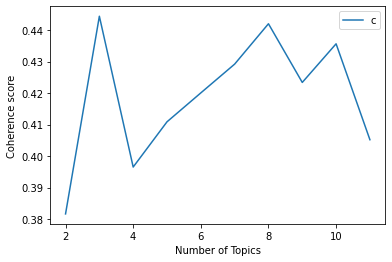
\includegraphics[width=1\textwidth]{
				resultLSA.png
			}
			\caption[Kết quả thuật toán LSA trong Topic Modeling]{
				Kết quả thuật toán LSA trong Topic Modeling 
			}
		\end{figure}
\end{enumerate}

\subsection{Latent Dirichlet Allocation (LDA)}
Model LDA là lớp mô hình sinh (generative model) cho phép xác định một tợp hợp các chủ đề tưởng tượng (imaginary topics) mà mỗi topic sẽ được biểu diễn bởi tập hợp các từ. Mục tiêu của LDA là mapping toàn bộ các văn bản sang các topics tương ứng sao cho các từ trong mỗi một văn bản sẽ thể hiện những topic tưởng tượng ấy.

\textbf{Ứng dụng của gensim trong bài toán LDA} \cite{WEBSITE:14}

Dữ liệu được sử dụng là 20-newgroups dataset

Dữ liệu bao gồm 11k các posts liên quan đến 20 chủ đề khác nhau đã được gán nhãn.

\begin{enumerate}
	\item \textbf{Import các thư viện cần thiết}
	\lstinputlisting[style=codePython]{"Code/importData.py"}
	
	\item \textbf{Dữ liệu mẫu} %\ref{tab:data}:
	\lstinputlisting[style=plaintext]{"Code/loadDataRes.txt"}
	
%	\begin{table}[h!]
%		\caption{Dữ liệu mẫu: }
%		\label{tab:data}
%		\centering
%		\begin{tabular}{l l l 1}
%			\toprule
%			\tabhead{No}&\tabhead{content}&\tabhead{target}&\tabhead{target_names}\\
%			\midrule
%			0 & From: lerxst@wam.umd.edu (where's my thing)... & 7 & rec.autos\\
%			1 & From: guykuo@carson.u.washington.edu (Guy Kuo)... & 4 & comp.sys.mac.hardware\\
%			10 & From: guykuo@carson.u.washington.edu (Guy Kuo)... & 8 & rec.motorcycles\\
%			100 & From: guykuo@carson.u.washington.edu (Guy Kuo)... & 6 & misc.forsale\\
%			1000 & 	From: dabl2@nlm.nih.gov (Don A.B. Lindbergh)... & 2 & comp.os.ms-windows.misc\\
%			\bottomrule \\
%		\end{tabular}
%	\end{table}
	
	\item \textbf{Visualization số lượng các topics}:
		\begin{figure}[h!]
			\centering
			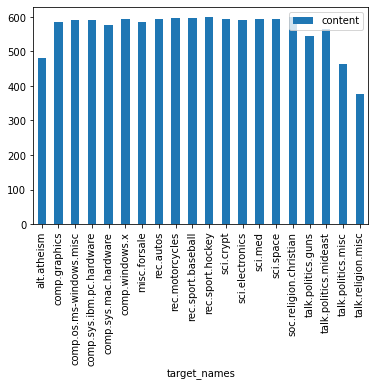
\includegraphics[width=1\textwidth]{
				output.png
			}
			\caption[Visualization số lượng các topics]{
				Visualization số lượng các topics
			}
		\end{figure}
		Như vậy có 20 nhóm, mỗi nhóm có số lượng các posts trong khoảng từ 400-600. phân về các chủ đề như: auto, mobile, medicine,….
	\newpage
	\item \textbf{Tiền xử lý dữ liệu}:
	\lstinputlisting[style=codePython]{"Code/preprocessing1.py"}
	\textbf{Kết quả}:
	\lstinputlisting[style=plaintext]{"Code/preprocessing1Res.txt"}
	
	\item \textbf{Tạo ra các bigram và trigram}:
	Hiện tại các từ vựng đang gồm toàn bộ là những từ đơn. Để tăng độ chính xác cho mô hình ta sẽ cần gom cụm các từ đơn có tần xuất xuất hiện cùng nhau chung thành những collocations có độ dài gồm 2 hoặc 3 từ. Ta sẽ gọi chúng là các bigram hoặc trigram
	\lstinputlisting[style=codePython]{"Code/bgramTrigramModel.py"}
	\textbf{Kết quả }: 
	\lstinputlisting[style=plaintext]{"Code/bgramTrigramModel.txt"}
	
	\item \textbf{Lọai bỏ các stopwords}: Loại bỏ các từ stopwords và chỉ lọc ra các từ vựng là các từ có tag từ loại là \textbf{[‘NOUN’, ‘ADJ’, ‘VERB’, ‘ADV’]}.
	\lstinputlisting[style=codePython]{"Code/deleteStopwords.py"}
	\textbf{Kết quả =}:
	\lstinputlisting[style=plaintext]{"Code/deleteStopwords.txt"}
	
	\item \textbf{Tạo các dictionary}: Từ điển (dictionary) và bộ văn bản (corpus) là 2 input chính cho model LDA
	\lstinputlisting[style=codePython]{"Code/dictionary.py"}
	
	\textbf{Kết quả }:
	\lstinputlisting[style=plaintext]{"Code/dictionary.txt"}
	
	Sau khi xử lý ta đã thu được 1 corpus là list các cặp (index, frequency) mã hóa các văn bản về index được qui định trong dictionary kèm theo tần suất xuất hiện của chúng trong văn bản. Để convert ngược lại từ index sang từ vựng ta sử dụng dictionary là id2word như sau.
	\lstinputlisting[style=codePython]{"Code/convert.py"}
	\textbf{Kết quả }:
	\lstinputlisting[style=plaintext]{"Code/convert.txt"}
	
	\item \textbf{Xây dựng model LDA và in ra các keywords tìm được}:
	\lstinputlisting[style=codePython]{"Code/buildModelLDA.py"}
	\textbf{Kết quả }:
	\lstinputlisting[style=plaintext]{"Code/ldaRes.txt"}
	Đối với topic 1 ta thấy biểu diễn của chúng là: \textbf{'0.019*"information" + 0.017*"file" + 0.015*"program" + 0.015*"include" + '
		'0.013*"system" + 0.013*"also" + 0.013*"available" + 0.011*"software" + '
		'0.011*"standard" + 0.010*"new"} có nghĩa rằng có 10 từ vựng quan trọng nhất đóng góp vào topic này bao gồm: 'imformation', 'file, 'program, 'include, 'system, 'also, 'available, 'software', 'standard', 'new'. Dựa vào cảm quan ta có thể biết được rằng topic này liên quan đến \textbf{CÔNG NGHỆ}.
	
	\item \textbf{Tìm ra topic chính của document}
	\lstinputlisting[style=codePython]{"Code/mainTopics.py"}
	\textbf{Kết quả}: \ref{mainTopics}
	\begin{figure}[h!]
		\centering
		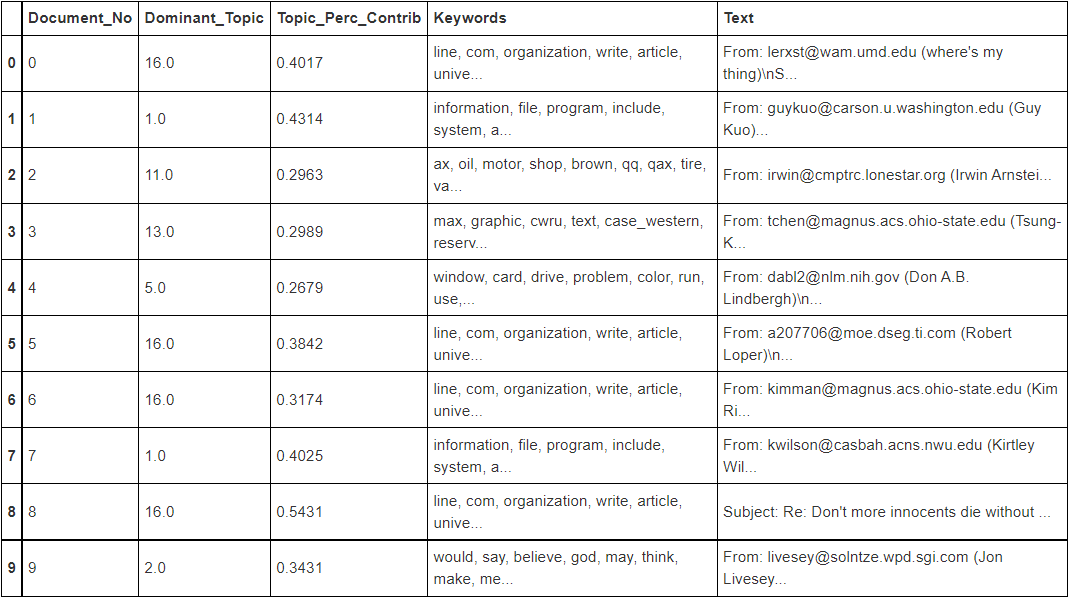
\includegraphics[width=1\textwidth]{
			mainTopics.png
		}
		\caption[Các topic chính của document sau khi được train bằng model LDA]{
			Các topic chính của document sau khi được train bằng model LDA  \label{mainTopics} \cite{WEBSITE:14}
		}
	\end{figure}
\end{enumerate}

\section{Kết luận}
Với bài toán Topic Modeling, việc xuất ra hết những từ/tài liệu quan trọng trong mỗi chủ đề không phải là điều tối ưu, đặc biệt với bộ dữ liệu lớn. Do vậy, giải pháp là ta chỉ hiển thị những từ/tài liệu thuộc top trong chủ đề. Điều này sẽ hữu ích nhất trong việc tìm được tên chủ đề. \cite{WEBSITE:15}
